% !TeX root = ../main_editorial.tex
\documentclass[../main_editorial.tex]{subfiles} % Inherits definitions from parent .tex file.

% Per-problem variable definitions
\newcommand{\problemName}{Balon Poligon}
\newcommand{\problemWriter}{William Gozali}
\newcommand{\problemEditorialWriter}{William Gozali}
\newcommand{\problemTags}{\textit{ternary search}, geometri}

\begin{document}

\begin{center}
    \section*{\problemName}
    \addcontentsline{toc}{section}{\problemName} % for pdf indexing
    
    \begin{tabular}{rl}
    Penulis soal : & \problemWriter \\
    Penulis editorial : & \problemEditorialWriter \\
    Penulis Solusi : & Pusaka Kaleb Setyabudi \\
    Tema : & \problemTags
    \end{tabular}
\end{center}

\subsection*{Catatan/Komentar}
\addcontentsline{toc}{subsection}{Catatan/Komentar} % for pdf indexing

Batasan kedua versi: $3 \le M \le 10; -10^6 \le X[i], Y[i] \le 10^6$

Untuk memudahkan penjelasan, digunakan definisi sebagai berikut:

\begin{enumerate}
  \item $O$ menyatakan titik $(0, 0)$.
  \item $T_1, T_2, ..., T_N$ sebagai titik-titik pada bidang Kartesius.
  \item $P_1, P_2, ..., P_{M-1}$ sebagai titik-titik sudut dari poligon.
  \item $\omega$ menyatakan besarnya sudut $\angle P_1OP_2$
\end{enumerate}

\subsection*{Versi Mudah}
\addcontentsline{toc}{subsection}{Versi Mudah} % for pdf indexing

Batasan: $\mathbf{N = 1}$

Solusi optimal dicapai apabila segmen garis $OT_1$ dijadikan garis yang tegak lurus terhadap $P_1P_2$.

\begin{figure*}[!h]
	\centering
	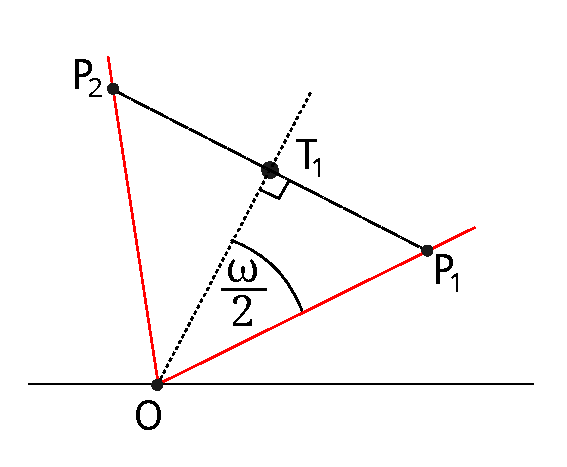
\includegraphics[width=0.35\textwidth]{balon/asset/easy.pdf}
\end{figure*}

Ukuran dari balon poligon adalah $||OP_1||$, yang dapat dicari dengan cara berikut:

\begin{eqnarray*}
||OT_1|| &=& ||OP_1|| \cos{\frac{\omega}{2}} \\
||OP_1|| &=& \frac{||OT_1||}{\cos{\frac{\omega}{2}}} \\
||OP_1|| &=& \frac{1}{\cos{\frac{\omega}{2}}} ||OT_1||
\end{eqnarray*}

\subsection*{Versi Sulit}
\addcontentsline{toc}{subsection}{Versi Sulit} % for pdf indexing

Batasan: $\mathbf{1 \le N \le 100}$

Untuk versi sulit, definisikan sebuah variabel tambahan, yaitu $\alpha$ yang menyatakan sudut yang dibentuk oleh sumbu-x positif terhadap $P_1$.

\begin{figure*}[!h]
	\centering
	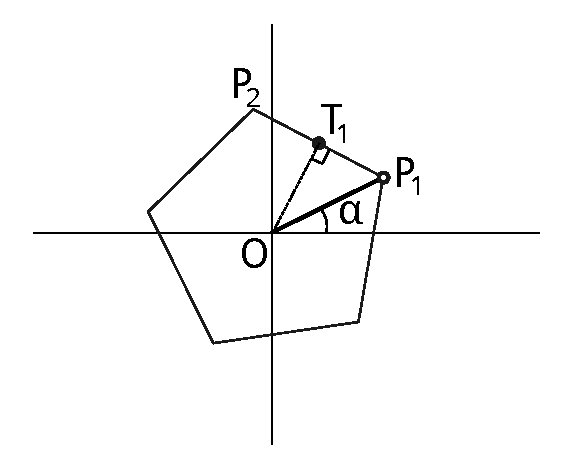
\includegraphics[width=0.35\textwidth]{balon/asset/hard-intro.pdf}
\end{figure*}

Karena poligon memiliki simetri putar, nilai $\alpha$ yang perlu dipedulikan adalah $0 \le \alpha < \omega$. 

Versi ini juga lebih mudah apabila kita bekerja dengan sistem koordinat kutub. Artinya, setiap titik $T_i$ memiliki dua informasi:

\begin{enumerate}
  \item Jarak $T_i$ ke titik $O$. Nyatakan nilai ini dengan $T_i^r$.
  \item Sudut yang dibentuk dari $T_i$, ke titik $O$, lalu menuju ke suatu titik $(\infty, 0)$. Nyatakan nilai ini dengan $T_i^\theta$. Nilai $T_i^\theta$ adalah anggota dari $[0, 360)$.
\end{enumerate}

Misalkan diberikan sebuah nilai $\alpha$, dan kita hendak menghitung berapa ukuran poligon apabila hanya terdapat titik $T_i$. Diketahui pula $T_i$ berada di dalam daerah yang diapit oleh $P_1$ dan $P_2$. 

Misalkan segmen garis $OQ$ merupakan segmen garis yang tegak lurus dengan $P_1$ dan $P_2$. Perhitungan nilai $||OP_1||$ dapat dicari dengan cara berikut:

\begin{eqnarray*}
||OP_1|| &=& \frac{1}{\cos{\frac{\omega}{2}}} ||OQ|| \\
&=& \frac{1}{\cos{\frac{\omega}{2}}} ||OT_i|| \cos{\left| \alpha + \frac{\omega}{2} - T_i^\theta \right|}
\end{eqnarray*}

\begin{figure*}[!h]
	\centering
	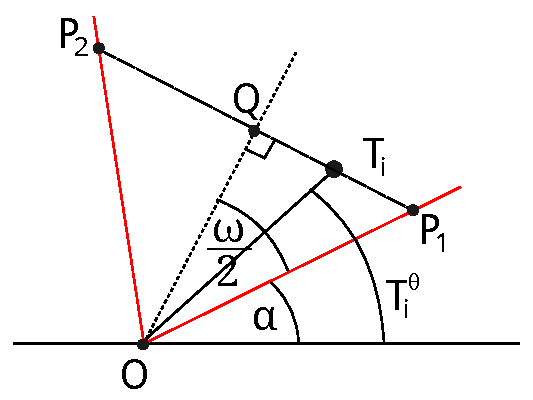
\includegraphics[width=0.35\textwidth]{balon/asset/hard-calc.pdf}
\end{figure*}

Untuk kasus ketika titik $T_i$ tidak berada di daerah yang diapit oleh $P_1$ dan $P_2$, normalisasi nilai $T_i^\theta$ dengan mengurangkannya dengan $\omega$ sampai berada di daerah yang diapit oleh $P_1$ dan $P_2$. Hasil perhitungan akan tetap benar, dikarenakan adanya simetri putar.

Apabila rumus ukuran poligon tersebut dinyatakan sebagai fungsi terhadap $\alpha$, yang mana terdefinisi untuk $0 \le \alpha < \omega$ maka fungsi tersebut akan membentuk suatu kurva yang memiliki tepat sebuah puncak dan sebuah lembah. Titik puncak dicapai ketika nilai $\alpha$ menyebabkan $T_i$ berada di posisi $Q$, dan titik terendah dicapai saat $\alpha$ menyebabkan $T_i$ berada di posisi $P_1$.

Misalkan $T_i^{min}$ menyatakan nilai $\alpha$ yang menyebabkan ukuran poligon paling kecil ketika hanya terdapat titik $T_i$. Nilai $\alpha$ yang memenuhi adalah nilai sebesar $T_i^\theta$ yang telah dinormalisasi.

Untuk kasus ketika hanya terdapat $T_1$, didapatkan kurva berikut, dengan $r$ menyatakan ukuran poligon:

\begin{figure*}[!h]
	\centering
	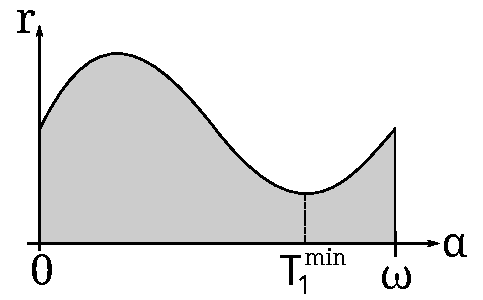
\includegraphics[width=0.35\textwidth]{balon/asset/hard-chart1.pdf}
\end{figure*}

Terdapat dua daerah yang mana masing-masing merupakan fungsi yang memiliki tepat sebuah nilai puncak, yaitu daerah $\alpha \in [0, T_1^{min}]$ dan $\alpha \in [T_1^{min}, \omega]$.

Untuk kasus ketika terdapat $T_1$ dan $T_2$, kita dapat mencari irisan kedua kurva tersebut:

\begin{figure*}[!h]
	\centering
	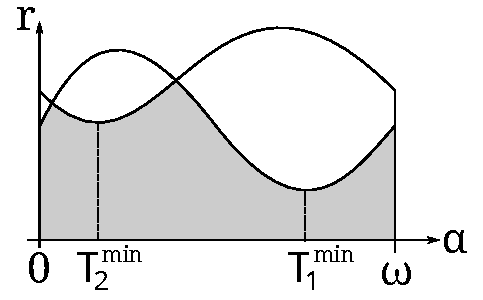
\includegraphics[width=0.35\textwidth]{balon/asset/hard-chart2.pdf}
\end{figure*}

Kini terdapat tiga daerah yang mana masing-masing merupakan fungsi yang memiliki tepat sebuah nilai puncak, yaitu daerah $\alpha \in [0, T_2^{min}]$, $\alpha \in [T_2^{min}, T_1^{min}]$, $\alpha \in [T_1^{min}, \omega]$.

Ketika seluruh kurva untuk $T_i$ digabungkan, didapatkan $\bigO{N}$ daerah yang masing-masing memiliki tepat sebuah nilai puncak. Lakukan \textit{ternary search} untuk masing-masing daerah tersebut, dan ambil nilai terbesar. Nilai ini adalah ukuran poligon terbesar yang mungkin.

Untuk akurasi, \textit{ternary search} dapat dilakukan sebanyak $k$ kali, misalnya antara 50 sampai dengan 100. Pada setiap tahap, diperlukan pemeriksaan terhadap nilai terkecil $r$ yang mungkin dari $N$ titik yang ada. Kompleksitas waktu untuk setiap \textit{ternary search} ini adalah $\bigO{kN}$. Karena dilakukan sebanyak $\bigO{N}$ kali, kompleksitas akhirnya adalah  $\bigO{kN^2}$.


\subsubsection*{Catatan Tambahan}

Terdapat solusi untuk versi sulit yang memiliki kompleksitas waktu $\bigO{N \log{N}}$, yaitu dengan melakukan \textit{binary search} pada ukuran poligon. Implementasi secara lebih rincinya diserahkan kepada pembaca sebagai latihan. 

\end{document}